\begin{sidewaysfigure}[htbp]
\centering 
  \subfloat[\acs{mus} = 0.1, \acs{mur} = 0.4, $v_{inlet}$ = 100 m/s .]
  {
	  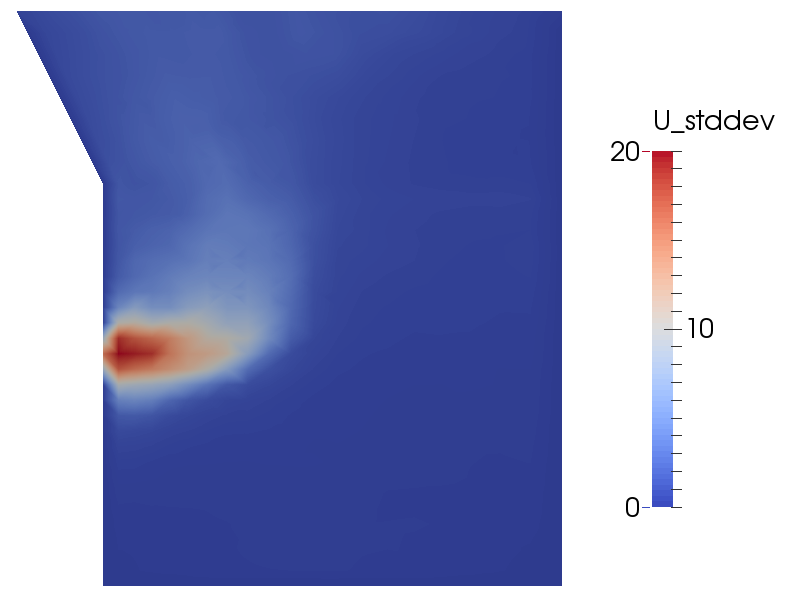
\includegraphics[width=.3\columnwidth]{images/229u_std_lf}
	  \label{fig:229u_std_lf}
  }
  \quad
    \subfloat[\acs{mus} = 0.5, \acs{mur} = 0.4, $v_{inlet}$ = 100 m/s .]
    {
	  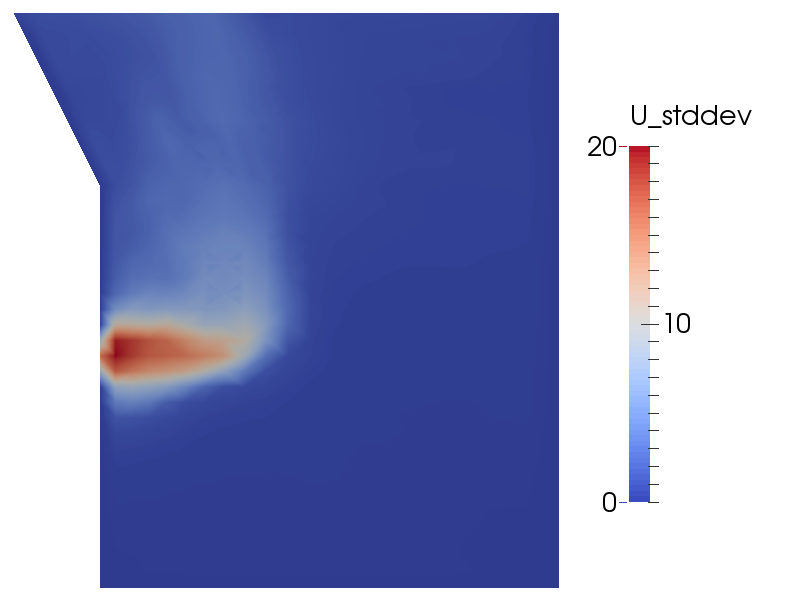
\includegraphics[width=.3\columnwidth]{images/245u_std_mf}
	  \label{fig:245u_std_mf}
  }
  \quad
    \subfloat[\acs{mus} = 0.9, \acs{mur} = 0.4, $v_{inlet}$ = 100 m/s .]
    {
	  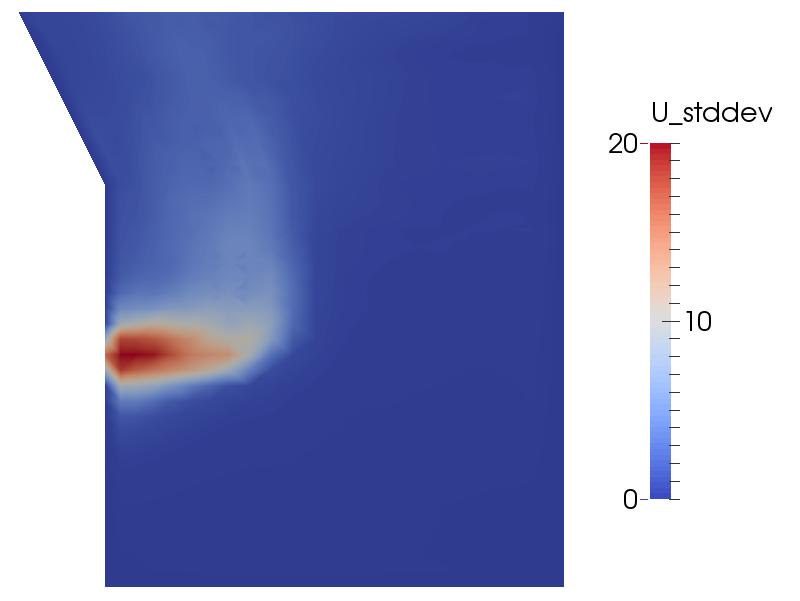
\includegraphics[width=.3\columnwidth]{images/228u_std_hf}
	  \label{fig:228u_std_hf}
  }
  \\
  \subfloat[\acs{mus} = 0.1, \acs{mur} = 0.4, $v_{inlet}$ = 200 m/s .]
  {
	  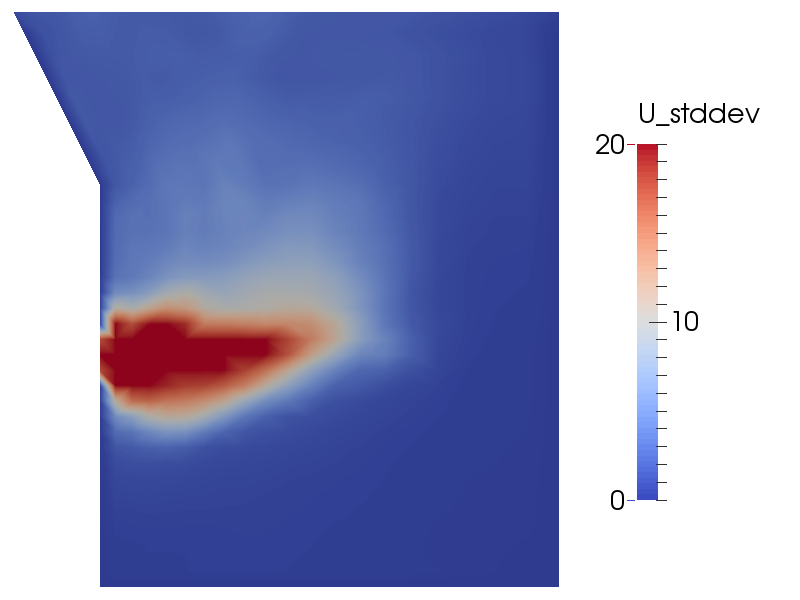
\includegraphics[width=.3\columnwidth]{images/244u_std_lfhv}
	  \label{fig:244u_std_lfhv}
  }
  \quad
    \subfloat[\acs{mus} = 0.9, \acs{mur} = 0.8, $v_{inlet}$ = 100 m/s .]
    {
	  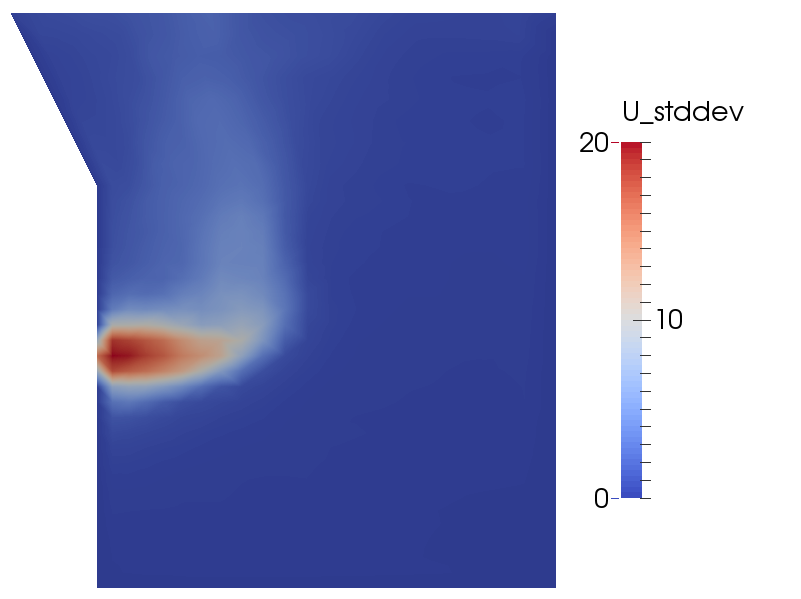
\includegraphics[width=.3\columnwidth]{images/243u_std_hfhr}
	  \label{fig:243u_std_hfhr}  }
  \\
  \caption{Standard deviation fluid velocity with different sliding friction
  coefficient.}
  \label{fig:258racewayustd}
\end{sidewaysfigure}